\section{\textbf{Introducci\'on}}
La habilidad de hacer predicciones acerca de acontecimientos o eventos de la vida real ha sido siempre un tema de gran inter\'es para la ciencia.\par 
En la \'ultima d\'ecada, la comunidad de miner\'ia de datos se ha interesado vehementemente en el hallazgo de patrones o reglas que puedan ser \'utiles en la predicci\'on de eventos de corto y de largo plazo \cite{main}.\par
La mayor\'ia de trabajos de investigaci\'on recientes, orientados en la predicci\'on de eventos de corto plazo mediante series temporales, se han enfocado principalmente en el an\'alisis de los \textit{\textbf{valores actuales}} del flujo de datos \cite{rulediscovery}\cite{subsequencematching}. Sin embargo, en una basta cantidad de casos, el an\'alisis de los valores actuales es irrelevante; en su lugar, la \textit{\textbf{forma}} actual del patr\'on o la regla motivo y la detecci\'on oportuna en el flujo de datos, pueden ayudar a vaticinar el futuro de forma m\'as precisa \cite{main}.\par
Este trabajo de investigaci\'on tiene como objetivo principal, la implementaci\'on de la medida de distancia llamada \textit{Cubic Spline Interpolation} en los algoritmos \textit{\textbf{\enquote{Rule Bit Saves}}} y \textit{\textbf{\enquote{Find Antecedent Candidates}}}, utilizados respectivamente en el hallazgo y la detecci\'on de reglas significativas, para llevar a cabo predicciones de corto plazo sobre series temporales complejas y en presencia de ruido.\par
Las predicciones de corto plazo sobre series temporales han tenido un auge importante, su aplicaci\'on y alcance se ha diversificado considerablemente. Las predicciones de corto plazo sobre texto durante las pulsaciones del teclado, predicciones sobre consultas de base de datos \cite{type}, predicciones sobre intervenciones m\'edicas \cite{medical}, son solo algunos ejemplos de predicciones sobre objectos discretos.\par
Recientemente, ha surgido una reto a\'un mayor; se requiere un mayor poder predictivo, lo que implica necesariamente la implementaci\'on de algoritmos de predicci\'on mucho m\'as precisos, m\'as veloces y que puedan hallar patrones sobre conjuntos de datos mucho m\'as grandes y complejos \cite{robotics}. Por ejemplo, el radar Doppler utilizado en las \'ultimas dos d\'ecadas para la detecci\'on de tornados, ha incrementado el tiempo promedio de alerta de 5.3 a 9.5 minutos, salvando un incontable n\'umero de vidas humanas a\~no con a\~no. Sin embargo, a\'un se reporta alrededor de un 26\% de tornados que no pueden predecirse mediante esta tecnolog\'ia \cite{weatherforcasting}. McGovern et al. argumentan en \cite{weatherprediction}, que las nuevas mejoras no vendr\'an necesariamente de sensores m\'as sofisticados, sino, de algoritmos de predicci\'on a\'un no inventados, que puedan examinar las series de tiempo actuales para hallar reglas predictivas.\par
Este documento se encuentra distribu\'ido de la siguiente manera: inicialmente, en la secci\'on dos, se desarrolla el marco te\'orico como un grupo de ideas y conceptos fundamentales que tiene como objetivo principal, guiar al lector en el marco de esta propuesta de investigaci\'on. En la segunda secci\'on, se exponen los detalles m\'as importantes de la propuesta de investigaci\'on, tales como el planteamiento del problema, la hip\'otesis, las m\'etricas utilizadas y del por qu\'e la importancia de llevar a cabo esta investigaci\'on. El objetivo general y los objetivos espec\'ificos de esta propuesta, se ofrecen en las secciones cuatro y cinco respectivamente. El alcance y las limitaciones del proyecto son puntualmente descritas en la secci\'on seis, mientras que los entregables ser\'an enlistados en la secci\'on siete. El dise\~no experimental y el ambiente de desarrollo comprenden la metodolog\'ia que se utilizar\'a m\'as adelante en el desarrollo de esta investigaci\'on, dentro del tiempo programado en el cronograma de actividades establecido en la secci\'on nueve del documento.
\section{\textbf{Marco Te\'orico}}
En la \'ultima decada ha surgido enorme inter\'es acerca de mineria de datos sobre series temporales. Literalmente, cientos de art\'iculos han introducido nuevos algoritmos para indexar, clasificar, segmentar y agrupar series temporales \cite{sigmod}. Es por lo anterior, que iniciamos el desarrollo del marco te\'orico definiendo series temporales, como una pieza de conocimiento angular para la comprensi\'on de nuestra propuesta de tesis.
\subsection{Series Temporales}
Las series temporales, pueden definirse como \textit{\enquote{una secuencia ordenada de N observaciones (datos) ordenadas y equidistantes cronol\'ogicamente, sobre una caracter\'istica (serie univariable o escalar) o sobre varias caracter\'isticas (serie multivariable o vectorial), de una unidad observable, en diferentes momentos}} \cite{tak-chung}.\par
Una representaci\'on matem\'atica com\'un de una serie temporal \textit{univariable} puede verse de la siguiente manera:\par
$y_1, y_2,...,y_N; (y_t)^N t=1; (y_t:t=1,...,N)$, donde $y_t$ es la observaci\'on $n^0$ $t(1 \leq t \leq N)$ de la serie y N es el n\'umero de observaciones que componen la serie completa (el tama\~no o la longitud de la serie) \cite{concepts}.\par
En el siguiente gr\'afico, se pueden observar algunos ejemplos de las diferentes formas que pueden adoptar las series temporales con respecto a la fuente de datos. Algunas, son m\'as predecibles y constantes, mientras que otras fluctuan con mayor frecuencia en amplitud o simplemente presentan mayor cantidad de ruido.
\begin{center}
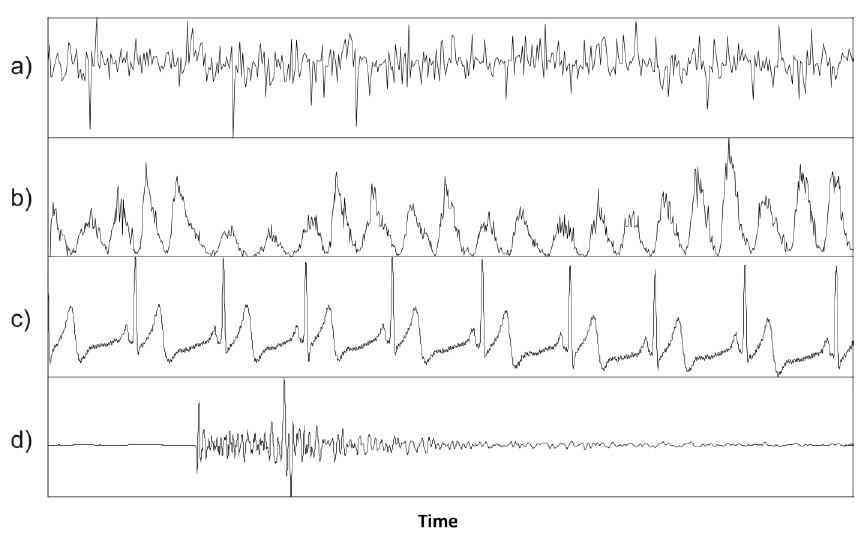
\includegraphics[scale=0.7]{timeSeries.png}\\
\vspace*{10pt}
\footnotesize{
\textbf{Figura 1.} Ejemplo de datos de series temporales relacionados con: \textbf{a)} Monz\'on, \textbf{b)} Manchas Solares, \textbf{c)} Electrocardiograma, \textbf{d)} Se\~nales S\'ismicas.
}\\ \textbf{Fuente:} \cite{concepts}.
\end{center}
La representaci\'on matem\'atica m\'as frecuente de una serie temporal multivariable, puede definirse de la siguiente manera:\par
$y_1, y_2,...,y_N; (y_t)^N t=1; (y_t: t=1,...,N)$, donde $y_t \equiv [y_t1, y_t2,...,y_tM]' (m \geq 2)$ es la observaci\'on $n^0$ $t(1 \leq t \leq N)$ de la serie y N es el n\'umero de observaciones que conforman la serie completa.\par
Las observaciones pueden ser almacenadas en una matriz $Y$ de orden $N X M$, como se muestra a continuaci\'on en la siguiente imagen:\\
\begin{equation}
Y \equiv \kbordermatrix{
				 & {    } \\	
				 & {y'_1} \\
				 & {y'_2} \\
				 & {.}    \\
				 & {.}    \\
 				 & {.}    \\
 				 & {y'_N} \\
		} \equiv
\kbordermatrix{
				 & {    }  & {    }   & {     } & {     } & {     } & {     }\\	
				 & {y'_{11}} & {y'_{12}}  & {  .  } & {  .  } & {  .  } & { y_{1M}}\\	
				 & {y'_{21}} & {y'_{22}}  & {  .  } & {  .  } & {  .  } & { y_{2M}}\\	
				 & {.}     & {.} &  &  &  & {.} \\
				 & {.}     & {.} &  &  &  & {.} \\
 				 & {.}     & {.} &  &  &  & {.} \\
 				 & {y'_{N1}} & {y'_{N2}} & {.} & {.} & {.} & {y_{NM}}  \\
}
\end{equation}\\
donde $y_{tj}$ es la observaci\'on $n^0$ $t(1 \leq t \leq N)$ sobre la caracter\'istica o variable $n^0$ $j(1 \leq t \leq N)$, que es la misma en todo momento $t$ \cite{concepts}.
\subsection{Aplicaci\'on y An\'alisis de Series Temporales}
La medici\'on y el seguimiento del comportamiento de alg\'un fen\'omeno o los datos espec\'ificos de alguna actividad en el tiempo, pueden producir informaci\'on muy relevante. Es informaci\'on de primera mano, que puede ser utilizada para comprender mejor aquello que ha venido ocurriendo, monitorear el estado actual para explicar la relaci\'on causal o la estructura subyacente que producen los datos observados, y finalmente, permite realizar predicciones o pron\'osticos que podr\'ian proveer un control anticipado sobre el fen\'omeno que se est\'a estudiando \cite{main}.\par
Muchas series temporales tienen una tendencia creciente, por ejemplo, el n\'umero de autom\'oviles en uso en casi todos los pa\'ises durante los \'ultimos cincuenta a\~nos, o decreciente como el n\'umero de personas que trabajan en la agricultura; otras sin embargo, no tienen tendencia y son estacionarias, por ejemplo, la luminosidad a horas sucesivas, que var\'ia c\'iclicamente a lo largo de las 24 horas del d\'ia.\par
Por otra parte, existe una amplia gama de aplicaciones, en campos como la medicina, el an\'alisis bursatil, la meteorolog\'ia, la geof\'isica, la astrof\'isica, entre muchas otras disciplinas, cuyas observaciones pueden ser representadas como series de tiempo. Dichas observaciones, pueden ser exploradas y analizadas mediante el uso de t\'ecnicas de \textit{mineria de datos}, por ejemplo, a trav\'es del descubrimiento de patrones y el agrupamiento (clustering), t\'ecnicas  de clasificaci\'on, el descubrimiento de reglas y el resumen o la abstracci\'on de los datos \cite{concepts}.\par
Como se explicar\'a m\'as adelante durante el desarrollo de este documento, la propuesta de investigaci\'on se enfoca principalmente en la mejora de dos algoritmos utilizados en el descubrimiento de reglas significativas sobre series temporales. \par 
Una \textit{\enquote{\textbf{regla significativa}}} debe entenderse como un patr\'on o \enquote{subsecuencia recurrente} de la serie de tiempo (usualmente llamado \textit{\textbf{motif}}), que describe un evento o comportamiento real del conjunto de datos. Una vez que el motif ha sido identificado, se debe analizar su capacidad predictiva en relaci\'on con el flujo de datos. Se debe tener presente el hecho de que no todas las reglas motif identificadas se convertir\'an necesariamente en reglas significativas \cite{main}.\par
A continuaci\'on, se exponen algunas de las principales dificultades que podr\'ian presentarse durante las diferentes etapas del proceso de  miner\'ia de datos sobre series temporales.
\subsection{Grandes Retos Sobre la Miner\'ia de Series Temporales}
El an\'alisis y el descubrimiento de patrones sobre series temporales, por definici\'on, presenta una serie de retos y complicaciones que deben abordarse, tales como: la super multidimensional, la presencia de grandes cantidades de datos que muchas veces resultan innecesarios o poco \'utiles durante el an\'alisis, la sensibilidad al ruido o a la presencia de valores at\'ipicos y el dinamismo durante la transmici\'on de datos o \textit{\enquote{data streaming}}, debido a que requiere un procesamiento de datos temporales a una gran velocidad, fluctuando const\'antemente y potencialmente infinitos \cite{main}.\par
Por otra parte, \textit{\textbf{el c\'alculo de la similitud}} durante la comparaci\'on de dos o m\'as series temporales es considerado un desaf\'io a\'un mucho m\'as crucial en la miner\'ia de series temporales, especialmente cuando se ha realizado previamente una reducci\'on de la dimensionalidad, de la escala o la amplitud a trav\'es del tiempo. La carencia de un alineamiento oportuno sobre el eje tiempo o la amplitud, durante el c\'alculo de la similitud entre dos o m\'as series temporales, es un problema serio porque tiene un impacto directo sobre el resultado de la comparaci\'on. \cite{concepts}.\par
El c\'alculo de la similitud es indispensable en la identificaci\'on de segmentos repetitivos contenidos en la serie de tiempo. Estos patrones se conocen como \textit{\textbf{\enquote{motivos}}} o \textit{\textbf{\enquote{motifs}}}, los cuales, pueden definirse como patrones o \textit{ocurrencias frecuentes de un subconjunto de la serie temporal} \cite{main}.\par
Los motifs pueden considerarse conocimiento puro o significativo, cuando como producto del minado de la serie temporal, se puede utilizar el \textit{motif} para explicar e incluso predecir, con una probabilidad, un fen\'omeno en el corto o el largo plazo.\par
La idenficaci\'on de reglas \textit{motif} se logra fundamentalmente apartir del c\'alculo de las medidas de distancia entre los elementos de dos o m\'as series temporales \cite{main}; la precisi\'on de dicho c\'alculo y el n\'umero de ocurrencias son vitales para determinar la calidad de dicha regla. Existen en la literatura, un n\'umero importante de medidas de distancia \cite{distancecomparison}. Las medidas de distancia m\'as importantes para la comprensi\'on de esta propuesta ser\'an desarrolladas a continuaci\'on.
\subsection{Medidas de Distancia para el C\'alculo de la Similitud}
Las medidas de similitud son de vital importancia cuando se requieren ejecutar tareas de an\'alisis y miner\'ia de datos sobre series temporales, tales como descubrimiento de patrones, agrupamiento, clasificaci\'on, descubrimiento de reglas, entre otras. Debido a la naturaleza n\'umerica y continuade de los datos caracter\'isticos de las series temporales, las medidas de similitud, t\'ipicamente se llevan a cabo en forma de aproximaciones.\par
La complejidad inherente al c\'alculo de las medidas de similitud, imponen normalmente las principales limitaciones y restricciones de capacidad y tiempo de c\'omputo, sobre los algoritmos utilizados en el an\'alisis y la miner\'ia de datos de series temporales \cite{algoanalysis}. Es decir, cuanto m\'as r\'apido y preciso sea el c\'alculo de la medida de similitud definida en el algoritmo, menor ser\'a el tiempo de c\'omputo necesario para la ejecuci\'on del procedimiento completo de miner\'ia de datos sobre las series temporales.\par
Para el desarrollo de este proyecto, se utilizar\'an espec\'ificamente cinco medidas de distancia: 1- Distancia Euclidiana, 2-  Swale, 3- Spade, 4- EPR y 5- Cubic Spline Interpolation. Cada una de las medidas de distancia se desarrollar\'a a continuaci'on.
\subsubsection{\textbf{Distancia Euclideana}}
La distancia Euclidiana es la \textit{distancia \enquote{ordinaria} entre dos puntos de un espacio eucl\'ideo} \cite{euclidean}. 
La distancia Euclideana tiene la caracter\'istica de ser la medida de distancia m\'as simple y la m\'as utilizada para comparar series temporales \cite{motifs}. Por ejemplo, si se require comparar dos series temporales $Q$ y $C$, de largo $n$, donde $Q = q_1, q_2, ..., q_i, ..., q_n$ y $C = c_1, c_2, ..., c_i, ..., c_n$, se puede utilizar la distancia Euclideana ob\'icua cuya f\'ormula matem\'atica es la siguiente: 
\begin{equation}
DE(Q, C) \equiv \sqrt[2]{\sum\limits_{i=1}^{n}ݍ{(q_i - c_i)}^2}
\end{equation}
Con se muestra en la \textbf{Figura 2}, la visualizaci\'on del c\'alculo de la distancia Euclideana puede verse entonces como la ra\'iz cuadrada de la suma de diferencia al cuadrado; tal y como se observa en cada l\'inea vertical para cada punto de datos desde $C$ hasta $Q$ y viceversa.
\begin{center}
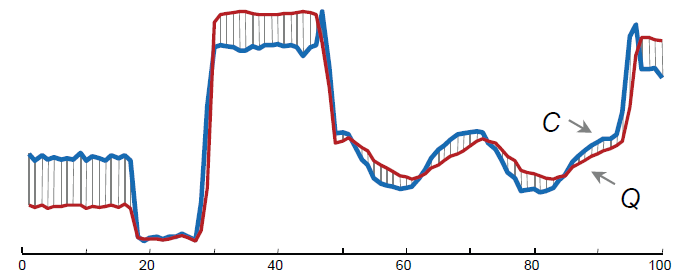
\includegraphics[scale=0.7]{euclidean.png}\\
\vspace*{10pt}
\footnotesize{\textbf{Figura 2.} Visualizaci\'on de la distancia Euclidiana entre dos series temporales C y Q.}\\ \textbf{Fuente:} \cite{euclidean}.
\end{center}
\subsubsection{DTW (Dynamic Time Warping)}
En el a\~no 1994, Berndt y Clifford \cite{dtw} proponen \textit{\textbf{\enquote{Dynamic Time Warping}}}. En el an\'alisis de series de tiempo, DTW es un algoritmo para medir el\'asticamente la similitud entre dos secuencias temporales que pueden variar en velocidad y por ende en alineamiento, en relaci\'on con el eje tiempo \cite{concepts}.\par A diferencia de la distancia Euclidiana, el c\'alculo de la similitud no se hace en forma lineal, por el contrario, las secuencias son \enquote{deformadas} de manera no lineal, para determinar la medida de similitud independiente con respecto a ciertas variaciones en el eje tiempo. Por ejemplo, la tarea de detecci\'on de patrones implica la b\'usqueda de una serie de tiempo $S$, para instancias de una plantilla $T$, donde $S = s_1, s_2, ..., s_i, ..., s_n$ y $T = t_1, t_2, ..., t_i, ..., t_n$.\par
Las secuencias $S$ y $T$, pueden ser acomodadas para conformar un plano de $m$ por $n$ o un cuadrante, en donde cada punto del cuadrante, $(i, j)$, corresponde a un alineamiento entre elementos $s_i$ y $t_i$.\par
Un camino $W$, alinea los elementos que pertenecen a $S$ y a $T$, tal que la distancia entre ellos es minimizada.\\
\begin{equation}
W = w_1, w_2, ..., w_k
\end{equation}
Es decir, $W$ es una secuencia o un camino espec\'ifico de puntos en el cuadrante, en donde cada $w_k$ corresponde a un punto $(i,j)_k$.
\begin{center}
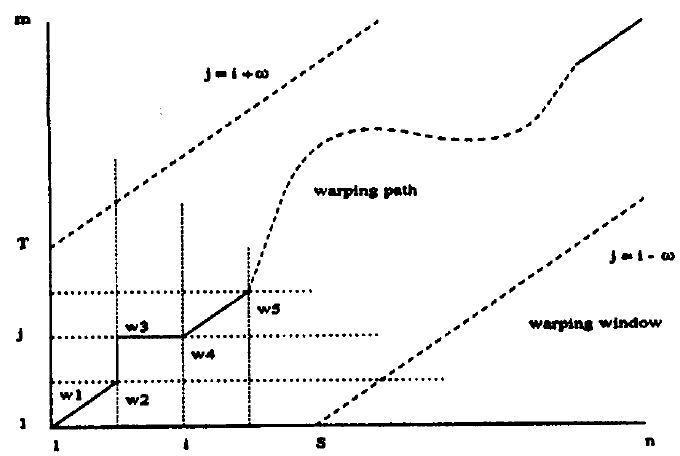
\includegraphics[scale=0.7]{dtw.png}\\
\vspace*{10pt}
\footnotesize{\textbf{Figura 3.} Visualizaci\'on de un camino w en un cuandrante de $m$ por $n$.}\\ \textbf{Fuente:} \cite{dtw}.
\end{center}
Posteriormente, por definici\'on, se debe definir una medida de distancia. En \cite{dtw}, los autores proponen $\delta(i,j) = (s_i - t_j)^2$. Una vez definida la medida de distancia, se puede definir formalmente DTW como la minimizaci\'on sobre los caminos o rutas potenciales no lineales, basados en la distancia acumulada para cada ruta, en donde $\delta$ es una medida de distancia entre dos puntos de datos o elementos de las series temporales.
\begin{equation}
DTW (S,T) = min_W[\sum\limits_{k=1}^{p}\delta(w_k)]
\end{equation}
En la Figura 4, se muestra observa un ejemplo claro de la forma que adoptan las deformaciones no lineales calculadas mediante el algoritmo DTW, para adaptar la diferencia de los puntos de datos con respecto al eje tiempo.
\begin{center}
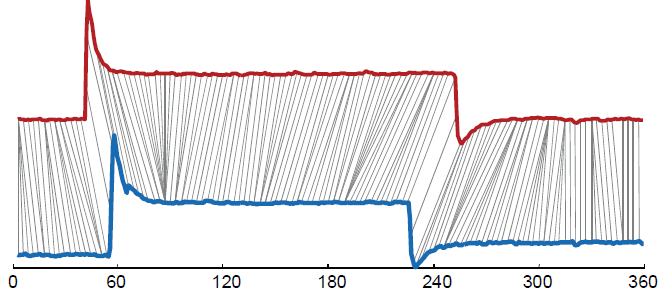
\includegraphics[scale=0.7]{dtw2.png}\\
\vspace*{10pt}
\footnotesize{\textbf{Figura 4.} Dos segmentos de series temporales acerca del comportamiento de insectos se alinean con invarianza a la deformaci\'on (\textit{\enquote{warping}}) ha sido computado mediante el uso de DTW.}\\ \textbf{Fuente:} \cite{dtw}.
\end{center}
\subsubsection{\textbf{Distancia \enquote{Swale}}}
En \cite{swale}, los autores proponen un modelo de similitud llamado \textbf{\textit{\enquote{Swale}}} (\enquote{\textit{Sequence Weighted ALignmEnt}}, por sus siglas en Ingl\'es); este modelo utiliza un sistema de puntuaci\'on para recompensar las similitudes y penalizar las disimilitudes durante la comparaci\'on de series temporales. El uso de \textit{Swale} requiere necesariamente el ajuste de tres par\'ametros: 1- un umbral de similitud \textbf{$\epsilon$}, 2- un valor o peso $r$ utilizado para recompensar las similitudes y 3- un valor o peso $p$ para penalizar los vacios o disimilitudes \cite{swale}.
\subsubsection{El Ruido y La Interpolaci\'on en Series Temporales}